\documentclass[border=3mm]{standalone}

\usepackage{tikz}
\usetikzlibrary{positioning,shapes.misc}
\usetikzlibrary{calc}
\usepackage{xcolor}

\def\centerarc[#1] (#2) (#3:#4:#5)% [draw options] (center) (initial angle:final angle:radius)
{ \draw[#1] (#2) ++(#3:#5) arc (#3:#4:#5);
}


\begin{document}

    
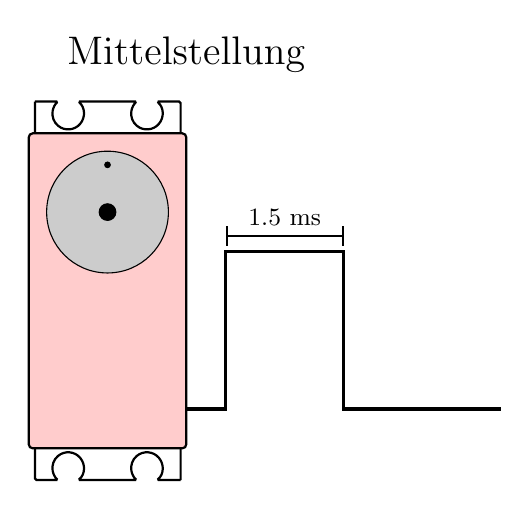
\begin{tikzpicture}
 %   \draw[step=1cm,gray,very thin]  (0,0) grid (6,6);
    \node (middle) at (3,6) {\Large Mittelstellung};
    \coordinate (c0) at (0.95,0.75);
    \coordinate (c1) at (1.5,0.75);
    \coordinate (c2) at (2.5,0.75);
    \coordinate (c3) at (2.8,0.75);    
    \coordinate (t0) at (0.95,5.25);
    \coordinate (t1) at (1.5,5.25);
    \coordinate (t2) at (2.5,5.25);
    \coordinate (t3) at (2.8,5.25);
    \draw[thick,rounded corners=0.2mm] ($(c3) + (-50:2mm)$) -- ($(c2) + (-50:2mm)$) arc (-50:230:2mm) -- ($(c1) + (-50:2mm)$) arc (-50:230:2mm) -- ($(c0) + (-50:2mm)$) -- ($(t0) + (50:2mm)$);
    
    \draw[thick,rounded corners=0.2mm]  ($(c3) + (-50:2mm)$) -- ($(t3) + (50:2mm)$) -- ($(t2) + (50:2mm)$) arc (50:-230:2mm) -- ($(t1) + (50:2mm)$) arc (50:-230:2mm) -- ($(t0) + (50:2mm)$) ;
    
    \draw [black, thick,rounded corners=0.5mm ,fill=red!20] (1,1) rectangle (3,5);  
    \coordinate (m) at (2,4);
    \filldraw[fill=black!20] (m) circle (22pt);
    \filldraw (m) circle (3pt);
    \filldraw ($(m)+ (90:0.6) $)circle (1pt);
  
  % PWM Signal  
  \draw[very thick] plot coordinates {(3,1.5) (3.5,1.5) (3.5,3.5) (5,3.5) (5,1.5) (7,1.5)};
  \draw[|-|,thick] (3.5,3.7) -- (5,3.7)
        node[midway, above]{\small 1.5 ms};   
  
\end{tikzpicture}

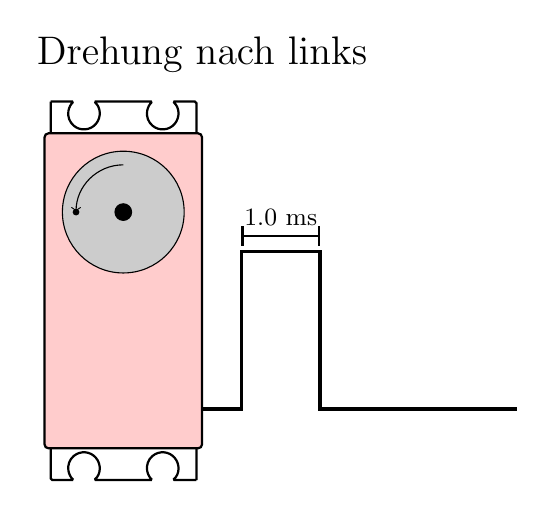
\begin{tikzpicture}
  %\draw[step=1cm,gray,very thin]  (0,0) grid (6,6);
  \node (links) at (3,6) {\Large Drehung nach links};
  \coordinate (c0) at (0.95,0.75);
  \coordinate (c1) at (1.5,0.75);
  \coordinate (c2) at (2.5,0.75);
  \coordinate (c3) at (2.8,0.75);    
  \coordinate (t0) at (0.95,5.25);
  \coordinate (t1) at (1.5,5.25);
  \coordinate (t2) at (2.5,5.25);
  \coordinate (t3) at (2.8,5.25);
  \draw[thick,rounded corners=0.2mm] ($(c3) + (-50:2mm)$) -- ($(c2) + (-50:2mm)$) arc (-50:230:2mm) -- ($(c1) + (-50:2mm)$) arc (-50:230:2mm) -- ($(c0) + (-50:2mm)$) -- ($(t0) + (50:2mm)$);
  
  \draw[thick,rounded corners=0.2mm]  ($(c3) + (-50:2mm)$) -- ($(t3) + (50:2mm)$) -- ($(t2) + (50:2mm)$) arc (50:-230:2mm) -- ($(t1) + (50:2mm)$) arc (50:-230:2mm) -- ($(t0) + (50:2mm)$) ;
  
  \draw [black, thick,rounded corners=0.5mm ,fill=red!20] (1,1) rectangle (3,5);  
  \coordinate (m) at (2,4);
  \filldraw[fill=black!20] (m) circle (22pt);
  \filldraw (m) circle (3pt);
  \filldraw ($(m)+ (180:0.6) $)circle (1pt);
  \draw[->] ($(m)+ (90:0.6) $) arc (90:180:0.6);
  % PWM Signal  
  \draw[very thick] plot coordinates {(3,1.5) (3.5,1.5) (3.5,3.5) (4.5,3.5) (4.5,1.5) (7,1.5)};
  \draw[|-|,thick] (3.5,3.7) -- (4.5,3.7)
        node[midway, above]{\small 1.0 ms};   
        
  \end{tikzpicture}

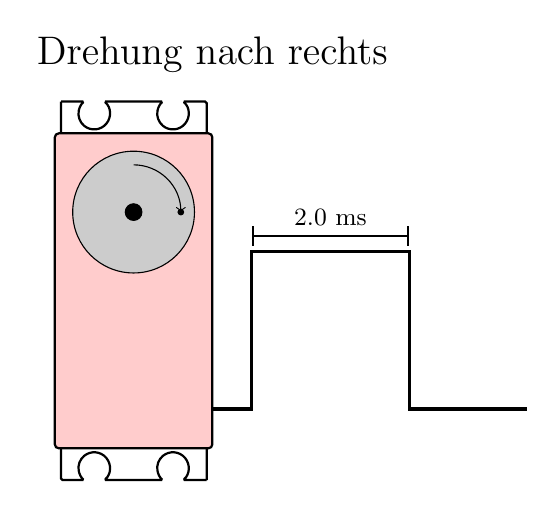
\begin{tikzpicture}
   % \draw[step=1cm,gray,very thin]  (0,0) grid (6,6);
  \node (rechts) at (3,6) {\Large Drehung nach rechts};
    \coordinate (c0) at (0.95,0.75);
    \coordinate (c1) at (1.5,0.75);
    \coordinate (c2) at (2.5,0.75);
    \coordinate (c3) at (2.8,0.75);    
    \coordinate (t0) at (0.95,5.25);
    \coordinate (t1) at (1.5,5.25);
    \coordinate (t2) at (2.5,5.25);
    \coordinate (t3) at (2.8,5.25);
    \draw[thick,rounded corners=0.2mm] ($(c3) + (-50:2mm)$) -- ($(c2) + (-50:2mm)$) arc (-50:230:2mm) -- ($(c1) + (-50:2mm)$) arc (-50:230:2mm) -- ($(c0) + (-50:2mm)$) -- ($(t0) + (50:2mm)$);
    
    \draw[thick,rounded corners=0.2mm]  ($(c3) + (-50:2mm)$) -- ($(t3) + (50:2mm)$) -- ($(t2) + (50:2mm)$) arc (50:-230:2mm) -- ($(t1) + (50:2mm)$) arc (50:-230:2mm) -- ($(t0) + (50:2mm)$) ;
    
    \draw [black, thick,rounded corners=0.5mm ,fill=red!20] (1,1) rectangle (3,5);  
    \coordinate (m) at (2,4);
    \filldraw[fill=black!20] (m) circle (22pt);
    \filldraw (m) circle (3pt);
    \filldraw ($(m)+ (0:0.6) $)circle (1pt);
    \draw[->] ($(m)+ (90:0.6) $) arc (90:0:0.6);
  % PWM Signal  
  \draw[very thick] plot coordinates {(3,1.5) (3.5,1.5) (3.5,3.5) (5.5,3.5) (5.5,1.5) (7,1.5)};
  \draw[|-|,thick] (3.5,3.7) -- (5.5,3.7)
        node[midway, above]{\small 2.0 ms};   
        
\end{tikzpicture}
 
 
\end{document}
